\documentclass{article}
\usepackage{tikz}
\usepackage{amsmath,amssymb,amsfonts,amsthm,bbm}
\usetikzlibrary{arrows}

\begin{document}

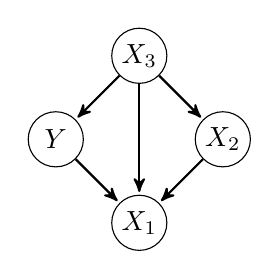
\begin{tikzpicture}[>=stealth', shorten >=1pt,
                             node distance=1.5cm, scale=1, 
                             transform shape, align=center, 
                             state/.style={circle, draw, minimum size=7mm, inner sep=0.5mm}]
            \node[state] (v2) at (0,0) {$X_1$};
            \node[state, above right of=v2] (v0) {$X_2$};
            \node[state, above left of=v2] (v1) {$Y$};
            \node[state, above right of=v1] (v3) {$X_3$};
            \draw [->, thick] (v0) edge (v2);
            \draw [->, thick] (v1) edge (v2);
            \draw [->, thick] (v3) edge (v1);
            \draw [->, thick] (v3) edge (v2);
            \draw [->, thick] (v3) edge (v0);
        \end{tikzpicture}

\end{document}